\section{Accelerated Sampling and Baseline Components}
\label{sec:critical}
% Generated from retained raw experiments; do not edit.
\newcommand{\SourceArrayMSE}{2.51\times10^{-8}}
\newcommand{\SourceMCMSE}{5.00\times10^{-7}}
\newcommand{\SourceRatio}{19.9}
\newcommand{\SourceArrayTime}{1.008}
\newcommand{\SourceMCTime}{0.073}
\newcommand{\NeighborRatio}{1.96}
\newcommand{\ShapeInitial}{1.35\times10^{-3}}
\newcommand{\ShapeMinimum}{1.41\times10^{-8}}
\newcommand{\ShapeMaximum}{9.39\times10^{-8}}
\newcommand{\SealedEigen}{2.24\times10^{-5}}


\begin{figure}[t]
 \centering
 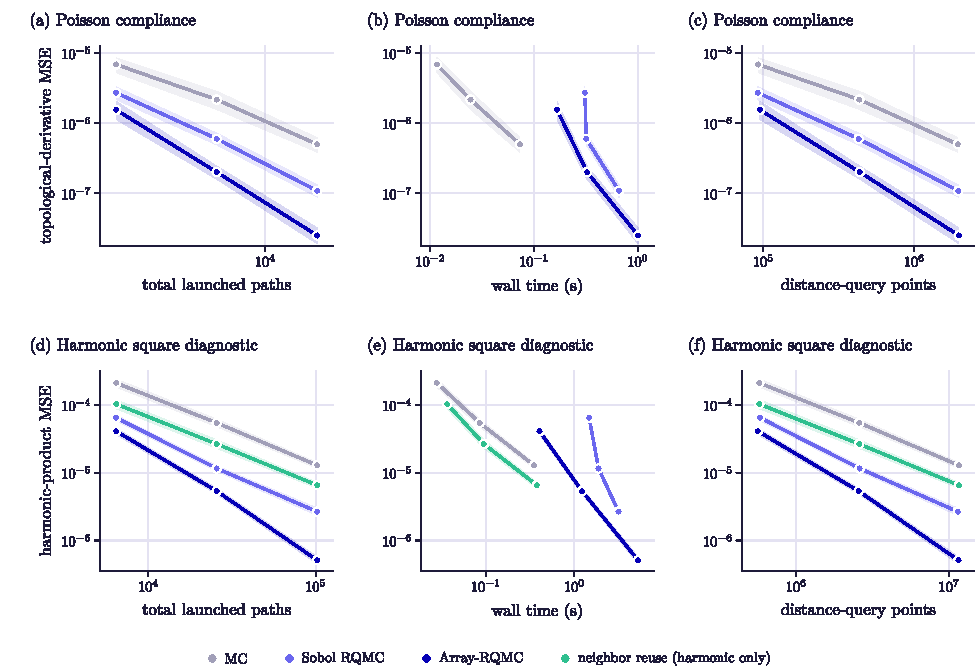
\includegraphics[width=0.975\textwidth]{figures/accelerated-sampling.pdf}
 \caption{Measured accelerated sampling with independent-batch cross-fitting.
 Top: the actual Poisson-compliance topological derivative on the disk.
 Bottom: a manufactured harmonic-product diagnostic on the square, including
 neighbor reuse.  All methods have equal launched-path budgets at corresponding
 markers.  The three columns expose the difference between statistical
 efficiency, Python wall time, and distance-query cost.  Bands describe
 uncertainty in empirical MSE across 32 independent full runs.}
 \label{fig:accelerated}
\end{figure}

\paragraph{A genuine Poisson-compliance derivative.}
On the unit disk, solve $-\Delta u=1$ with homogeneous Dirichlet data and
$J=\int_\Omega u$.  Then $p=u=(1-|z|^2)/4$ and
$D_T(z)=-(1-|z|^2)^2/16$.  Each WoS ball contributes the exact
constant-source Green integral $r^2/4$, with the same implementation for MC,
scrambled-Sobol RQMC, and shifted-Korobov Array-RQMC~\cite{ho2026array}.
We use five fixed sites, four independently randomized batches, 64, 256,
or 1,024 paths per batch, and 32 complete replications at each setting.
All products are cross-fitted across batches, as required by
\cref{app:batchindependence}; trajectories inside an array are never treated
as independent samples.  The shell tolerance is $10^{-7}$, and exhaustion of
the 256-step cap raises an error.  The maximum marginal truncation bias is
$\varepsilon/2$ here; it is not silently equated with zero.

At 1,024 paths per batch, Array-RQMC has mean TD MSE
$\SourceArrayMSE$ versus $\SourceMCMSE$ for MC, a
$\SourceRatio\times$ reduction at equal launched-path budget.
The corresponding median times are $\SourceArrayTime$ s and
$\SourceMCTime$ s.  Thus the measured Python implementation trades lower
error per path for substantial sorting overhead.  It establishes no uniform
runtime advantage.  RNG initialization and distance queries are included;
the timing applies only to these implementations and scenes.
The final Poisson campaign runs without other benchmark jobs; harmonic
timings come from a shared runtime and are exploratory.
\Cref{fig:accelerated} reports error against paths, time, and query count;
bands are percentile bootstrap intervals for mean MSE across the 32 full
replications, not certified insertion intervals.

\paragraph{Neighbor reuse on harmonic diagnostics.}
On both disk and square, we reuse the manufactured harmonic polynomials from
the earlier field diagnostic at 25 fixed sites in $[-0.55,0.55]^2$.
These nonzero-boundary harmonic pairs test the product-estimator algebra;
they are not the state and homogeneous-boundary adjoint of the Poisson
compliance problem above.  We implement the deterministic variance-bound
weights in Czekanski et al.~\cite{czekanski2026neighbors}, equations (17)--(18),
and retain the first sphere exit and final boundary value of every walk.
Both queries and weights are computed inside each independent batch.
At the largest square budget, neighbor reuse reduces product MSE by
$\NeighborRatio\times$ relative to MC using the same launched paths.
Our 13-bit Hilbert implementation matches the authors' Array-RQMC update
routine in four common-randomization cases to within $10^{-12}$.
We do not apply terminal-only neighbor reweighting to a source PDE:
its first-ball source contribution would need a separate correct treatment.

\begin{figure}[t]
 \centering
 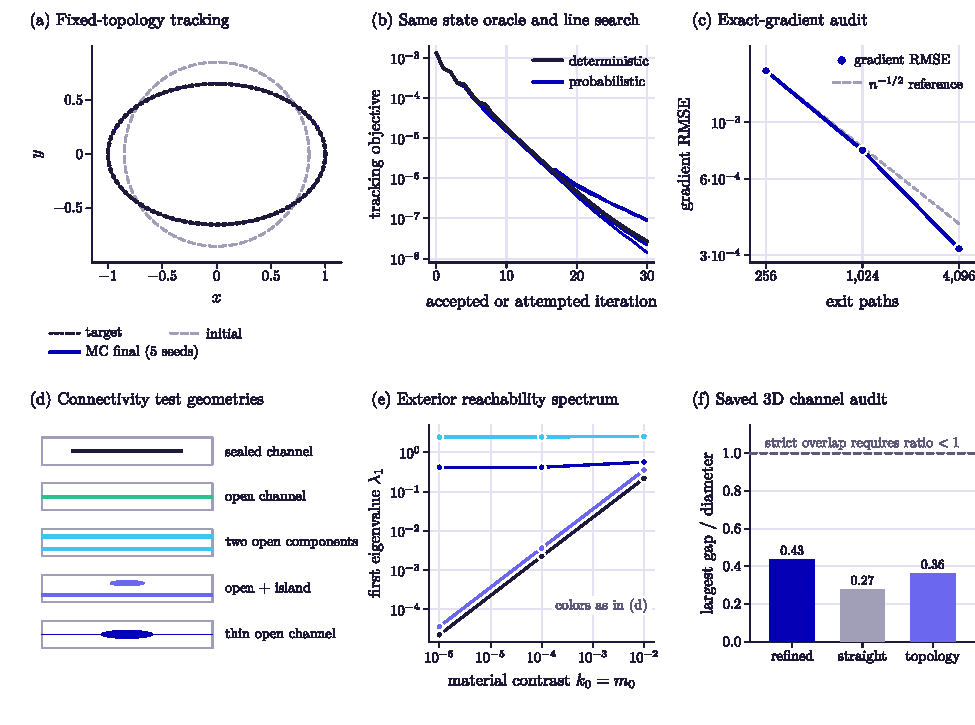
\includegraphics[width=0.985\textwidth]{figures/baseline-diagnostics.pdf}
 \caption{Baseline components and geometric feasibility.  (a--c) Exact-state
 ellipse tracking tests the probabilistic shape derivative and descent, with
 five stochastic runs.  (d--e) The reproduced two-phase spectral operator
 distinguishes sealed islands from exterior-connected voids; two open
 components are allowed.  (f) Existing 3D ball-chain designs satisfy the newly
 explicit strict-overlap guard.  These are component experiments, not complete
 PINN/FEM or level-set optimizer reproductions.}
 \label{fig:baselinecomponents}
\end{figure}

\paragraph{Fixed-topology probabilistic shape control.}
We specialize a probabilistic derivative~\cite{schmidt2026first}
to a two-parameter ellipse family, giving both optimizers the same exact
Poisson state.  The target has semiaxes $(1,0.65)$; the initial semiaxes are
$(0.85,0.85)$.  We compare the uniform-start, importance-weighted exit formula
with a separately derived deterministic pullback gradient
(\cref{app:shapeoracle}).  The deterministic gradient agrees with central
differences to within $10^{-8}$; 48 replications at each of three path budgets
audit the stochastic error.  With identical bounds and Armijo line searches,
five stochastic 30-step runs reduce the tracking objective from
$\ShapeInitial$ to the range $[\ShapeMinimum,\ShapeMaximum]$.
This validates the shape-derivative implementation on a fixed-topology design
task.  It does not measure neural-state training, boundary FEM smoothing,
or the complete published optimizer, and does not compare full optimizers.

\paragraph{Spectral connectivity reproduction and geometry correction.}
We reproduce the two-phase Dirichlet eigenproblem of
Andrade et al.~\cite{andrade2026connectivity}, equation (4), with $P_1$
triangles and consistent mass.  The cavity coefficients are $k_1=m_1=1$;
the other phase has $k_0=m_0\in\{10^{-2},10^{-4},10^{-6}\}$.
Five geometries and three mesh resolutions produce 45 eigenproblem solves.
At the finest $129\times129$ node resolution and contrast $10^{-6}$,
the sealed connected strip has $\lambda_1\approx\SealedEigen$, while
one open strip and two disconnected open strips both have
$\lambda_1\approx2.47$.  The latter is close to the limiting mixed-boundary
value $\pi^2/4$.  Thus their constraint tests exterior reachability, which is
different from connectedness of our interior channel.  At nonzero contrast,
even an isolated cavity has a positive eigenvalue; a threshold needs its own
contrast and resolution study.

After each radius recalibration, consecutive balls must overlap strictly. All three retained designs satisfy this check, with maximum gap/diameter ratios from $0.275$ to $0.434$. The geometric guarantee and its exterior-access limitation are proved in \cref{app:ballchain}.
\Cref{fig:baselinecomponents} separates these validation results from the
complete application comparisons, which were not performed for these two external methods.
